% \subsection{Cache-Aware Speculative Sampling}
\subsection{Balancing Cache Hit and Acceptance Rate with \Sys Sampling}
\label{sec:cache_sampling}



The majority of the time, the bonus token is sampled from the \textit{residual distribution} (except when all tokens are accepted, in which case it is sampled from the target directly). Recall the residual distribution is given by \(r(\cdot) \propto \max\left(p_{\mathrm{target}}(\cdot)-p_{\mathrm{draft}}(\cdot), 0\right)\).
This distribution can be difficult to predict, especially as sampling temperatures increase. 
We introduce a novel sampling scheme that makes this residual easier to predict and therefore increases cache hit rates. 

This sampling scheme exploits the fact that the residual distribution is a function of the draft distribution (which includes the draft sampling scheme).
We make the bonus token easier to predict by explicitly increasing the residual probability mass on the most likely draft tokens; and this is done by \textit{decreasing} the corresponding probability mass when sampling from the draft. 
In biasing the draft distribution, however, we may decrease the acceptance rate by having moved the draft distribution farther from the target (see \ref{thm:l1}), inducing a tradeoff between the acceptance rate and the cache hit rate, both of which contribute to end-to-end speed (see Figure \ref{fig:c-sweep}, left).
We show in Appendix~\ref{app:saguaro_construction} that there exist distributions $p_{\mathrm{target}}, p_{\mathrm{draft}}$ for which biasing the draft distribution in this way leads to end-to-end speedups.

\subsubsection{Algorithm}
\label{sec:cache_sampling_alg}

\begin{definition}
We define a \textbf{sampling scheme} as a function $\sigma\colon\mathbb{R}^V \rightarrow \Delta^{V-1}$ from model logits $z_{\mathrm{draft}} \in \mathbb{R}^V$ to a probability distribution $p\in \Delta^{V-1}$.
\end{definition}

To understand how to design a sampling scheme that increases the residual probability mass on the most likely draft tokens, we first note that the probability of token $t$ in the residual distribution is proportional to $\max(p_{\mathrm{target}}(t) - p_{\mathrm{draft}}(t), 0)$.
Thus, \textit{decreasing} $p_{\mathrm{draft}}(t)$  \textit{increases} the probability of $t$ in the residual.
This is exactly what our cache-aware sampling scheme does.

\begin{definition}
Given draft logits $z\in \mathbb{R}^V$, we define the \textbf{\Sys sampling scheme} $\sigma_{F,C}(z)$ for fan-out $F$ and downweighting constant $C \in [0, 1]$ as
\begin{eqnarray*}
\sigma_{F,C}(z) \propto  \begin{cases} 
C\cdot \exp\Big(z_t\Big)& \text{if } t \in \text{top}_F(z) \\ \exp\Big(z_t\Big)& \text{otherwise,}
\end{cases}
\end{eqnarray*}
% where $D$ is selected such that:
% \begin{eqnarray*}    
%  \sum_t \exp\Big(z_t\Big) &=&  \sum_{ t \in \text{top}_F(z)} C \cdot \exp\Big(z_t\Big) + \sum_{ t \notin \text{top}_F(z)} D \cdot \exp\Big(z_t\Big)
% \end{eqnarray*}
\end{definition}

In practice, $C$ is a hyperparameter that is chosen empirically. 



\subsubsection{Theoretical Results}
\label{sec:cache_sampling_theory}

\begin{theorem}
\label{thm:cache_sample}
For fan-out $F$ and primary speculator logits $z$, the cache hit rate $p_{\mathrm{hit}}$ of the \Sys sampling scheme increases monotonically as $C \rightarrow 0$.
\end{theorem}

The new sampling hyperparameter $C$ allows a trade-off between cache hit rate and acceptance rate. We plot this tradeoff in Figure \ref{fig:c-sweep} (left).
Figure \ref{fig:c-sweep} (right) presents an illustration of how \Sys sampling allows control of the \textit{residual distribution} by manipulating the draft distribution during speculation. 
% \color{red}
The intuition here is that \Sys sampling deliberately suppresses the draft probabilities on the $F$ cached tokens.  
By downweighting $p_{\mathrm{draft}}(t)$ on this set, the residual $\max\!\big(p_{\mathrm{target}}(t) - p_{\mathrm{draft}}(t),\,0\big)$
is pushed to \textit{concentrate} on those same tokens, \textit{increasing} the chance that the bonus token lands inside the cache by construction. 


\subsubsection{Empirical Evaluation}
We show in Figure~\ref{fig:c-sweep} how there is a trade-off between acceptance rate and cache hit rate which we can navigate by using the \Sys sampling scheme with different values of $C$. Lower values of $C$ lead to higher cache hit rates and lower acceptance rates as they bias the draft distribution away from the target to control the residual distribution.
% In Figure~\ref{fig:c-bars}, we see that to maximize speedup at larger temperatures it is important to sacrifice some acceptance rate (by choosing $C \ll 1$) to attain higher cache hit rates.
\color{black}

\begin{figure}[ht]
    \centering
    % \includegraphics[width=\linewidth]{figures/unified_cache_analysis_and_schematic.pdf}
    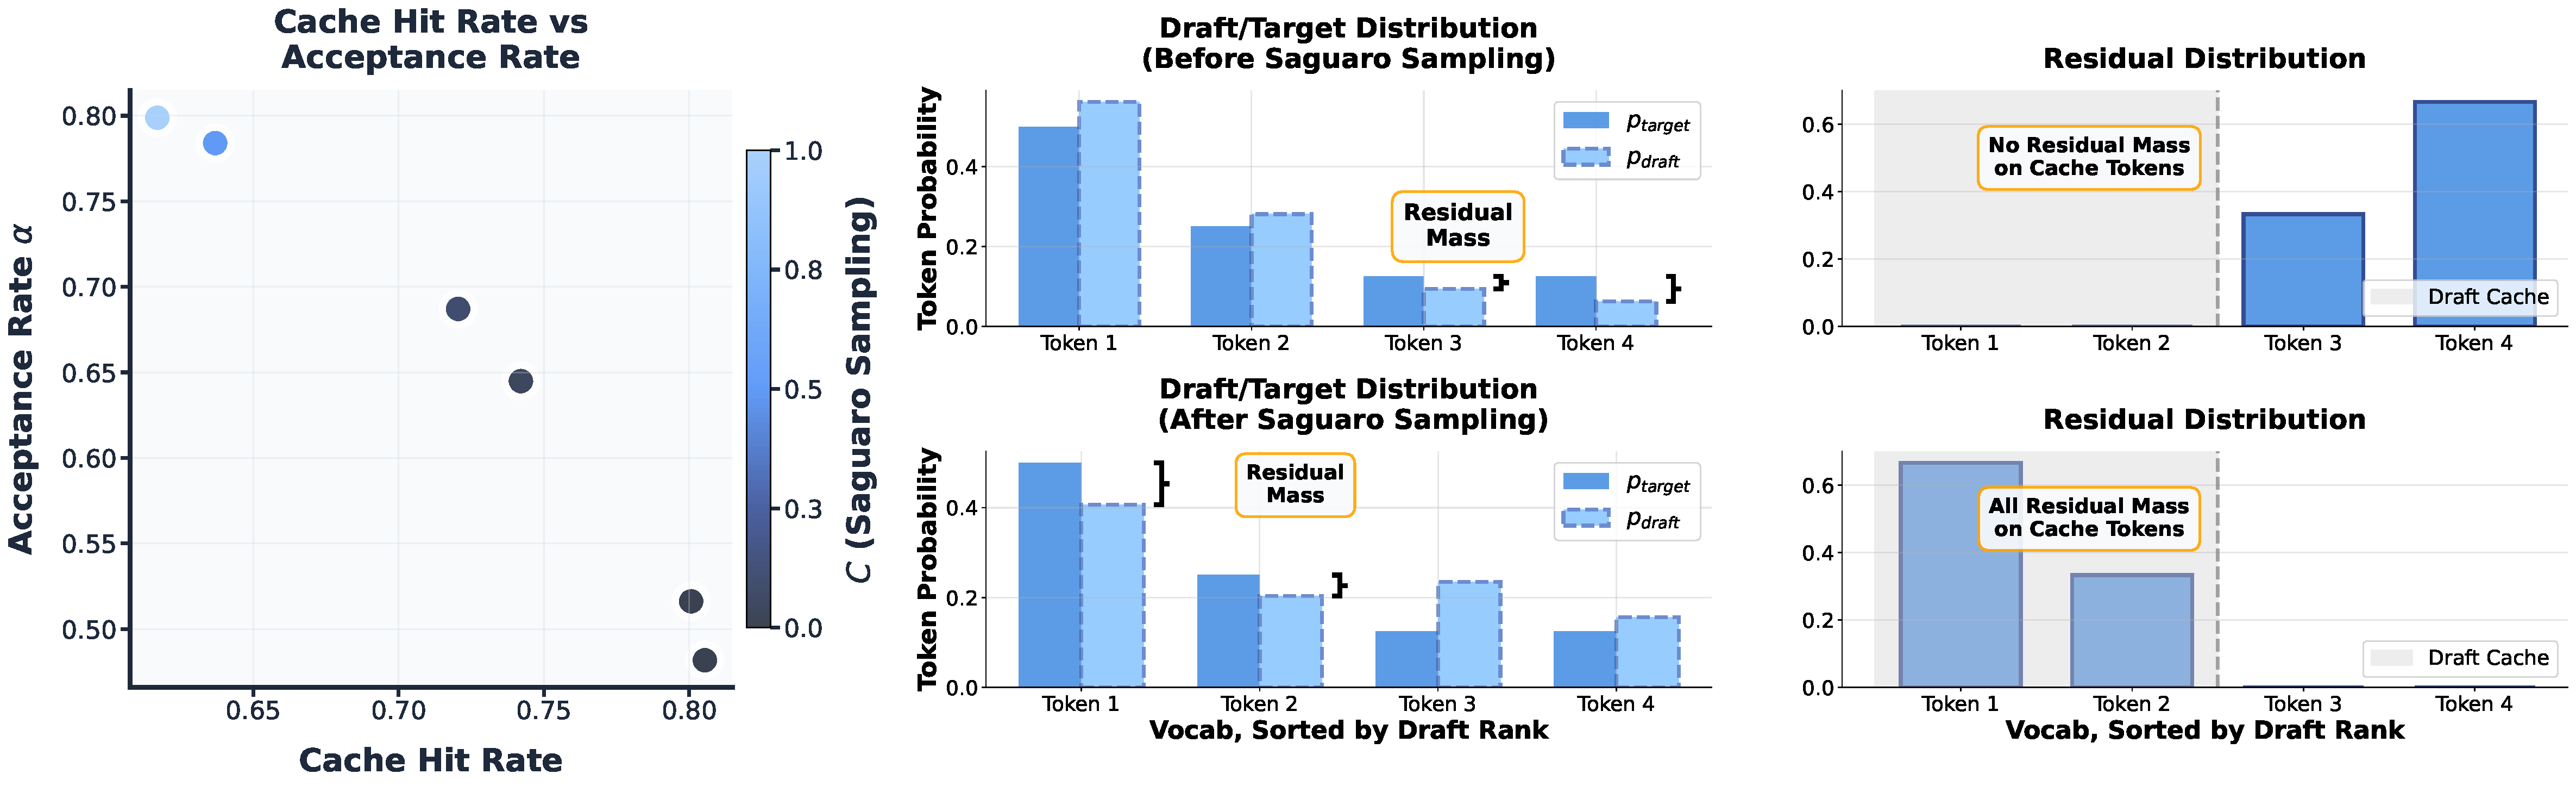
\includegraphics[width=\linewidth]{figures/unified_cache_hit_and_saguaro_plots.pdf}
    
    \caption{We introduce \Sys sampling, a novel sampling scheme designed specifically for SSD. (Left) It interpolates between high cache hit rate and high speculative acceptance rate. (Right) Illustrative schematic for how \Sys sampling increases residual probability mass on the top draft tokens, encouraging the sampled bonus token to lie in the speculation cache by construction. }
    \label{fig:c-sweep}
\end{figure}
